%!TEX root = ../thesis.tex
%*******************************************************************************
%*********************************** Fifth Chapter *****************************
%*******************************************************************************

\chapter{Results and Analysis}  %Title of the Fifth Chapter

\ifpdf
    \graphicspath{{Chapter1/Figs/Raster/}{Chapter1/Figs/PDF/}{Chapter1/Figs/}{/Users/luyolomagangane/Documents/Academics/Images/Recursive-Neural-Tensor-Networks/}}
\else
    \graphicspath{{Chapter1/Figs/Vector/}{Chapter1/Figs/}}
\fi


\section{Hypotheses Validation}
\dots and some more \dots
% Background on 3 hypotheses that were tested
In this chapter we evaluate three hypothesis explored in latent feature modelling for link prediction. Latent feature modelling has traditionally relied on linear modelling techniques in order to constrain parameterisation for computational efficiency at the expense of model expressiveness i.e. models that suffer from high bias. Recently nonlinear approaches have been proposed to overcome the bias problem and each propose hypothesis that aim to take advantage of their distinct architecture. The first nonlinear model to gain surpass state-of-the-art tensor factorisation models, was the recursive neural tensor network \cite{refefence}. There are two hypotheses proposed that were proposed in using this model architecture for link prediction, namely that recursive architectures are useful in part of speech tagging \cite{reference}, as the perform a combinatorial analysis of word sequences in sentences, instead of the conventional linear sequence used in part of speech tagging \cite{reference}. The second hypothesis is that pre-trained word embeddings offer superior performance to randomly generated entity vectors which were commonly used at the time for tensor factorisation \cite{reference}. \newline
The second hypothesis we explored is the use of convolutional hyper networks with relational factorisation for link prediction \cite{reference}. This research is the current state-of-that-art latent feature modelling technique for link prediction \cite{reference}. There are also two hypotheses explored in this research - the first is that convolutional filters can be used explicitly for relational factorisation \cite{reference}, the second is that the hyper network architecture is useful in generating the relational filters due to increased parameterisation using a hyper linear layer \cite{reference}. \newline
The final hypothesis we explored is the use of contextual entity representations as input to convolutional hyper networks. State-of-the-art natural language modelling techniques makes use contextual word representations \cite{Elmo, Bert} instead of static word embeddings \cite{fasttext, GloVe, Word2Vec}. Contextual word embeddings are represented as distinct subject entity representations, and distinct object entity representations. \newline
The following chapter presents the results and analysis from the experiments performed to validate these hypotheses.

\section{Recursive Neural Tensor Networks}
\dots and some more \dots
% Recursive neural tensor network 
Tensor factorisation has been a popular approach applied to latent feature modelling \cite{reference, reference, reference}. in order to improve model expressiveness, a Recursive Neural Tensor Network architecture was proposed \cite{reference}. This model is inspired by recursive neural networks \cite{reference}. Recursive neural networks have been applied to natural language processing tasks, particularly part of speech tagging \cite{reference}. Traditionally recurrent neural networks have been applied to this task \cite{reference}. Recurrent neural networks are based on the Markov assumption \cite{reference}, where the future states of the process depends only on the present state, not on the sequence of events that preceded it \cite{reference}. The state is constructed using sequential input within a time step window, for example, a sentence will contain a sequence of words, and the window will be the last word in the sentence and the four previous words before an anchor word. The state consists of the four previous words before the anchor word, and along with the anchor word, can be used to predict the next word in the sequence.\newline
Instead of producing a state using a sequence of previous words, recursive neural networks generate the state using a combinatorial tree of the word sequence. The number of potential combinations are dependent on the length of the sequence for example, a three word sequence has three combinations, a four word sequence has six combinations and  a five word sequence has ten combinations. The combinations which produce the smallest magnitudes are then filtered out from the network, and remaining combinations are then recombined as new combinations, This filtering and recombination process is then continued until a next word prediction is made. \newline
Recursive neural networks are combined with tensor factorisation to produce a more expressive model for link prediction. The subject and object entities are concatenated and then an matrix multiplication is taken with the resultant vector before a bias is added. \newline
% Contrastive Max Margin loss
The contrastive max-magrin loss \cite{reference} is used to train the RTNT model. The input consists of an entity-relational pair, where the entity is a subject entity. An object entity is presented as a target to complete the triple. A non-related object entity is presented is then presented as a corrupt object entity. Fact score is then computed for the target triple, as well as the corrupt triple as logits, and the difference between the two logits is the contrast between the true and false facts. The task is for the model is then to produce a higher fact score for the true triple than the false triple. If the model gets it wrong, then loss is generated and back propagated through the network to update model parameters. \newline

The link prediction accuracy results of the RNTN model, a nonlinear factorisation model compared against linear factorisation models, are presented in table 5.1:

\begin{table}[H]
\caption{Link prediction accuracy on Wordnet and Freebase}
\centering
\begin{tabular}{lllllllllll}
  \textbf{Model} & \textbf{Wordnet} & \textbf{Freebbase} & \textbf{Avg} \\
  \hline
  Distance Model & .683 & .610 & .647 \\
  Hadamard Model & .800 & .688 & .744 \\
  Single Layer Model & .760 & .853 & .807 \\
  Bilinear Model & \textbf{.841} & \textbf{.877} & \textbf{.859} \\
  Recursive Neural Tensor Network & .732 & .518 & .625 \\

\end{tabular}
\end{table}

% Susceptible to overfitting and early stopping solution
Machine learning models can suffer from overfitting \cite{reference} - when training has progressed too long, and the model parameters have been optimised for prediction on the training set. This leads to poor generalisation  and reveals itself in the form of increasing training accuracy, and decreasing validation accuracy. In order to overcome this problem, early stopping is often used during training. This is when triaining is terminated should decreasing validation accuracy be detected.\newline
% Hyperparameter optimisation
\begin{center}
    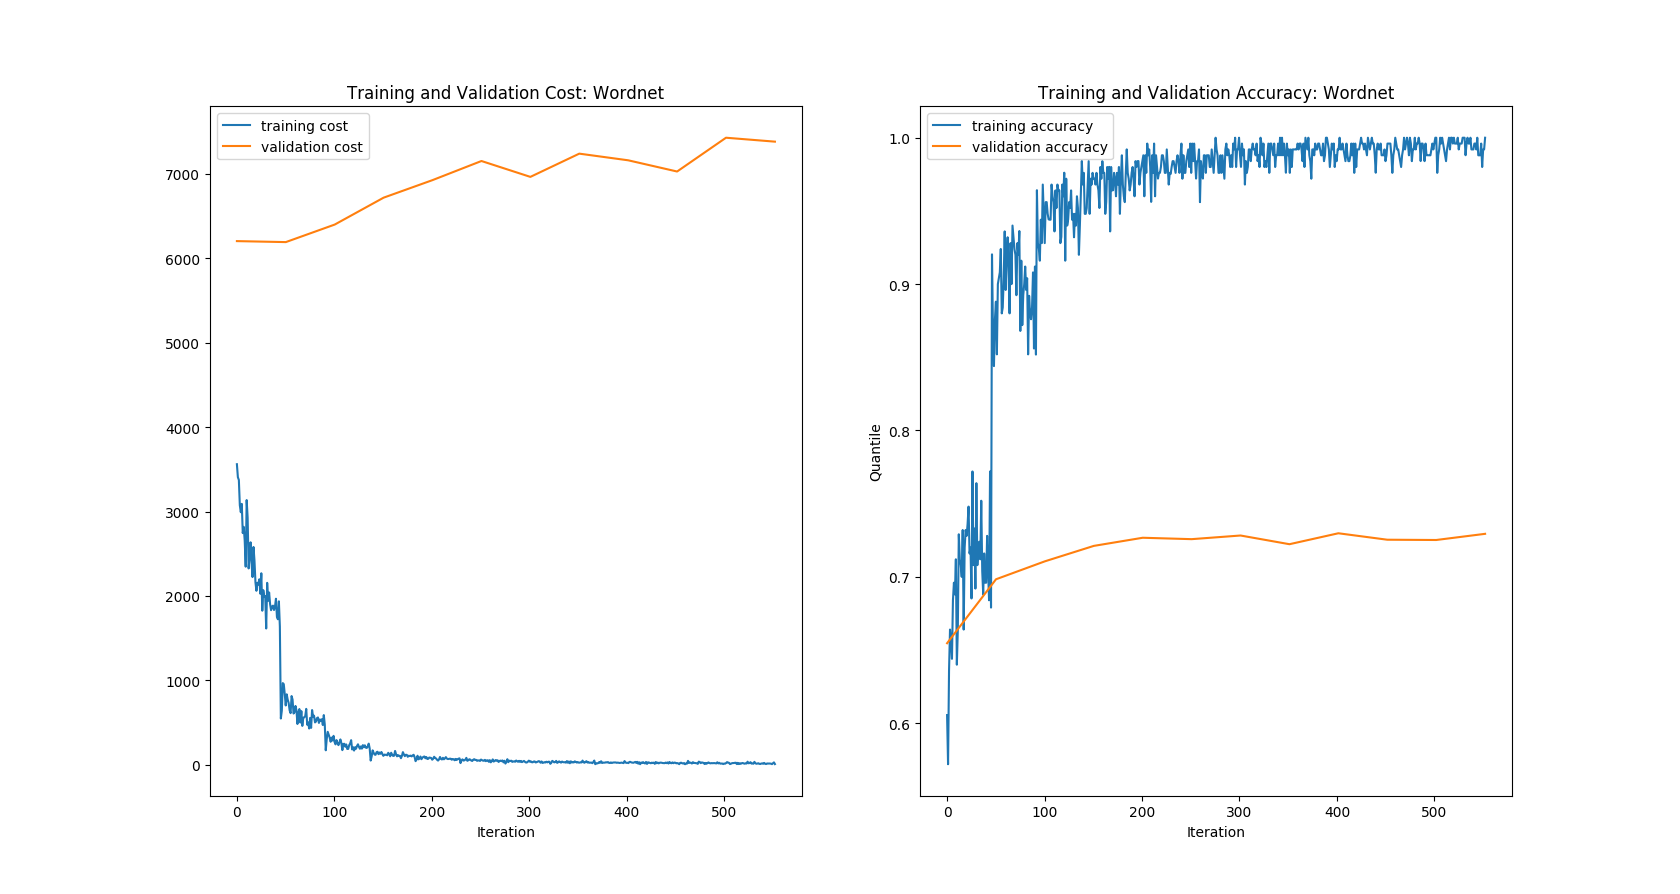
\includegraphics[width=\textwidth]{RNTN_Training_Results_Wordnet.png}
\end{center}

\begin{center}
    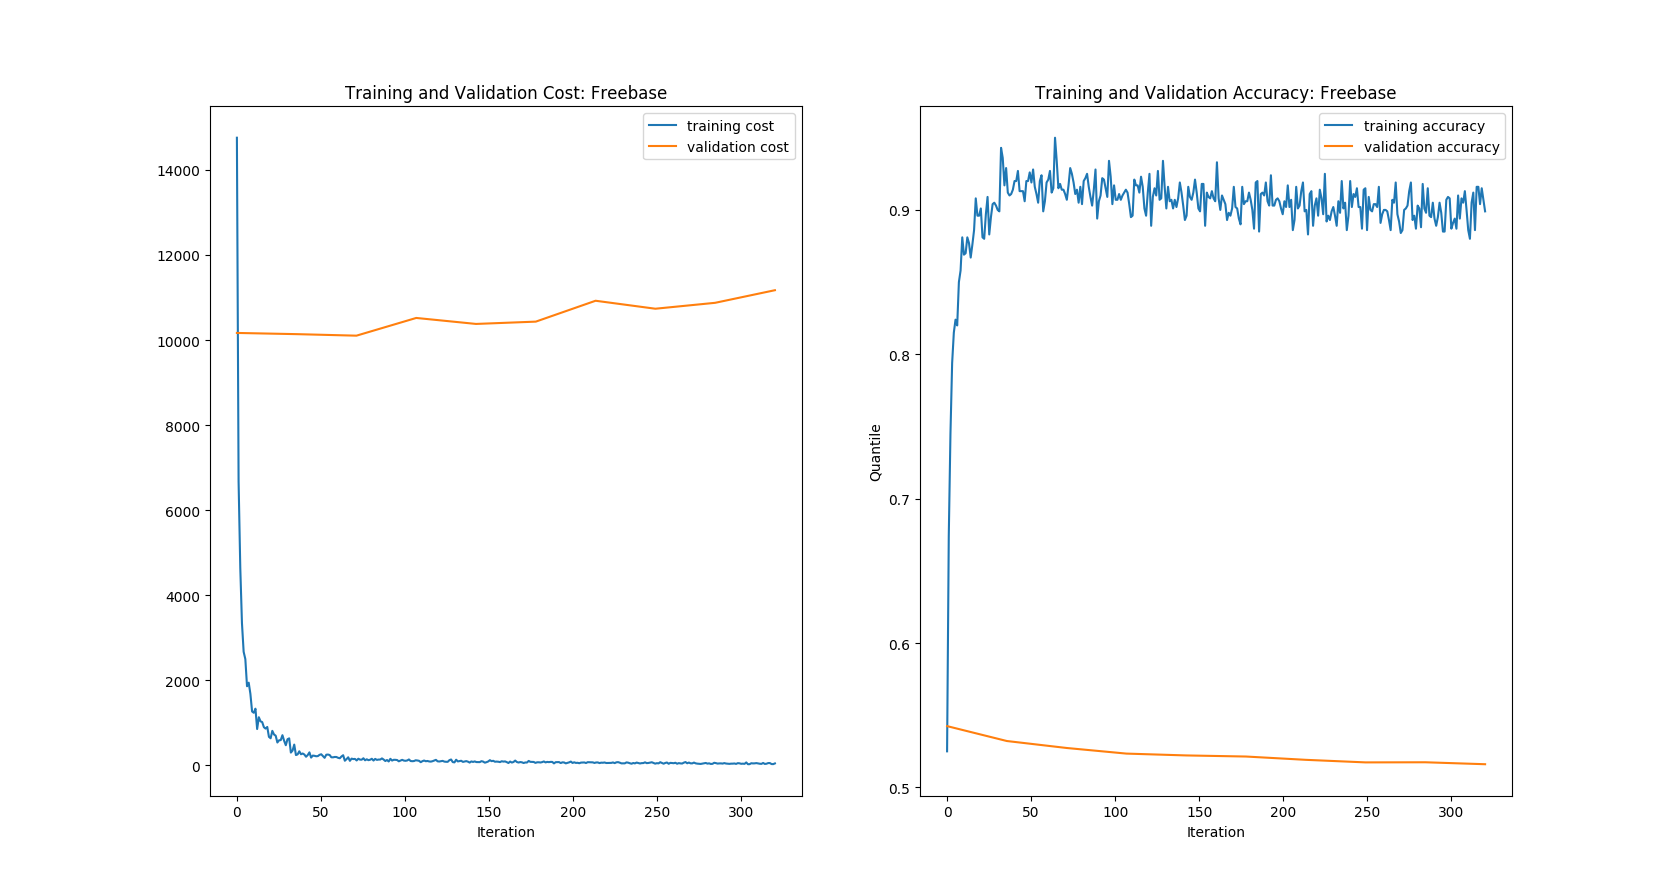
\includegraphics[width=\textwidth]{RNTN_Training_Results_Freebase.png}
\end{center}






\section{HypER Convolutional Neural Networks}

\section{HypER Convolutional Neural Networks with Contextual Entity Embeddings}

\section{Leader Board Research Versus Hypothesis Research}

